\documentclass[11pt]{article}
\usepackage{classTools}
\usepackage{xcolor}
\usepackage{minted}
\usepackage{graphicx}

\begin{document}

\psHeader{3}{Wed Oct. 4, 2023 (11:59pm)}

\textbf{Your name: } Cory Zimmerman

\textbf{Collaborators: } None

\textbf{No. of late days used on previous psets: } 0

\textbf{No. of late days used after including this pset: } 0


The purpose of this problem set is to solidify your understanding of the RAM model (and variants), and the relations between the RAM model, the Word-RAM model, Python programs, and variants. In particular, you will build skills in simulating one computational model by another and in evaluating the runtime of the simulations (both in theory and in practice).



\begin{enumerate}
 
    \item (Simulation in practice: RAMs on Python)  
    In the Github repository, we have given you a partially written Python implementation of a RAM Model simulator.  Your task is to fill in the missing parts of the code to obtain a complete RAM simulator.
     Your simulator should take as input a RAM Program $P$ and an input $x$, and simulate the execution of $P$ on $x$, and return whatever output $P$ produces (if it halts).  The RAM Program $P$ is given as a Python list $[v,C_0,C_1,\ldots,C_{\ell-1}]$, where $v$ is the number of variables used by $P$.  For simplicity, we assume that the variables are named $0,\ldots,v-1$ (rather than having names like ``tmpptr'' and ``insertvalue''), but you can introduce constants to give names to the variables.  The $0$\textsuperscript{th} variable will always be $\inputlen$, the $1$\textsuperscript{st} variable $\outputpointer$, and the $2$\textsuperscript{nd} variable $\outputlen$.  A command $C$ is given in the form of a list of the form $[\cmd]$, $[\cmd,i]$, $[\cmd,i,j]$, or $[\cmd,i,j,k]$, where $\cmd$ is the name of the command and $i,j,k$ are the indices of the variables or line numbers used in the command.  For example,  the command $\var_i = M[\var_j]$ would be represented as $(\READ,i,j)$.  See the Github repository for the precise syntax as well as some RAM programs you can use to test your simulator.

     \begin{quote}
         \color{purple}
         \begin{minted}{python}
def executeProgram(programArr, inputArr):
    setupEnv(programArr, inputArr)

    programArr = programArr[1:]
    programCounter = 0
    while programCounter < len(programArr):
        # Store the command and the list of operands.
        cmd = programArr[programCounter][0]
        ops = programArr[programCounter][1:]

        # Assignment commands
        if cmd == "read":
            # ['read', i, j]: lookup the var_j location in memory and assign that value to var_i
            variableList[ops[0]] = memory[variableList[ops[1]]]
        if cmd == "write":
            # ['write', i, j]: store the value of var_j in memory at the location var_i
            memory[variableList[ops[0]]] = variableList[ops[1]]
        if cmd == "assign":
            # ['assign', i, j]: assign var_i to the value j
            variableList[ops[0]] = ops[1]

        # Arithmetic commands
        if cmd == "+":
            # ['+', i, j, k]: compute (var_j + var_k) and store in var_i
            variableList[ops[0]] = variableList[ops[1]] + variableList[ops[2]]
        if cmd == "-":
            # ['-', i, j, k]: compute max((var_j - var_k), 0) and store in var_i.
            variableList[ops[0]] = max(variableList[ops[1]] - variableList[ops[2]], 0)
        if cmd == "*":
            # ['*', i, j, k]: compute (var_j * var_k) and store in var_i.
            variableList[ops[0]] = variableList[ops[1]] * variableList[ops[2]]
        if cmd == "/":
            #  ['/', i, j, k]: compute (var_j // var_k) and store in var_i.
            # Note that this is integer division. You should return an integer, not a float.
            # Remember division by 0 results in 0.
            if variableList[ops[2]] == 0:
                variableList[ops[0]] = 0
            else:
                variableList[ops[0]] = max(
                    variableList[ops[1]] // variableList[ops[2]], 0
                )

        # Control commands
        if cmd == "goto":
            # ['goto', i, j]: if var_i is equal to 0, go to line j
            if variableList[ops[0]] == 0:
                programCounter = ops[1]
                continue

        programCounter += 1

    # Return the memory starting at output_ptr with length of output_len
    return [
        memory[i] for i in range(variableList[1], variableList[1] + variableList[2])
    ]
         \end{minted}
     \end{quote}

    \item (Empirically evaluating simulation runtimes and explaining them theoretically)  

Consider the following two RAM programs:

\begin{algorithm}[H]
\Input{A single natural number $N$ (as an array of length 1)}
\Output{$17^{2^N+1}$ (as an array of length 1)}
\Variables{$\inputlen, \outputpointer, \outputlen, \counter, \result$}
\setcounter{AlgoLine}{-1}
$\zero = 0$\;
$\one = 1$\;
$\seventeen = 17$\;
$\outputlen = 1$\;
$\outputpointer = 0$\;
$\result = 17$\;
$\counter = M[\zero]$\;
\Indp
 IF $\counter == 0$ GOTO \ref{line:done}\; \label{line:loop}
$\result = \result \times \result$\;
$\counter = \counter - \one$\;
IF $\zero == 0$ GOTO \ref{line:loop}\;
\Indm
$\result = \result \times $\seventeen\; \label{line:done}
$M[\outputpointer]=\result$\;
\end{algorithm}

\begin{algorithm}[H]
\Input{A single natural number $N$ (as an array of length 1)}
\Output{$17^{2^N+1} \bmod 2^{32}$ (as an array of length 1)}
\Variables{$\inputlen, \outputpointer, \outputlen, \counter, \result, \temp, \W$}
\setcounter{AlgoLine}{-1}
$\zero = 0$\;
$\one = 1$\;
$\seventeen = 17$\;
$\outputlen = 1$\;
$\outputpointer = 0$\;
$\result = 17$\;
$\W = 2^{32}$\;
$\counter = M[\zero]$\;
\Indp
IF $\counter == 0$ GOTO \ref{line:done2}\; \label{line:loop2}
$\result = \result \times \result$\;
$\temp = \result / \W$\;
$\temp = \temp \times \W$\;
$\result = \result - \temp$\;
$\counter = \counter - \one$\;
IF $\zero == 0$ GOTO \ref{line:loop2}\;
\Indm
$\result = \result \times \seventeen$\;
\label{line:done2}
$\temp = \result / \W$\;
$\temp = \temp \times \W$\;
$\result = \result - \temp$\;
$M[\outputpointer]=\result$\; 
\end{algorithm}


\begin{enumerate}
    \item Exactly calculate (without asymptotic notation) the RAM-model running times of the above algorithms as a function of $N$.
    Which one is faster? \label{itm:RAMtime}    
    \begin{quote}
        \color{purple}
        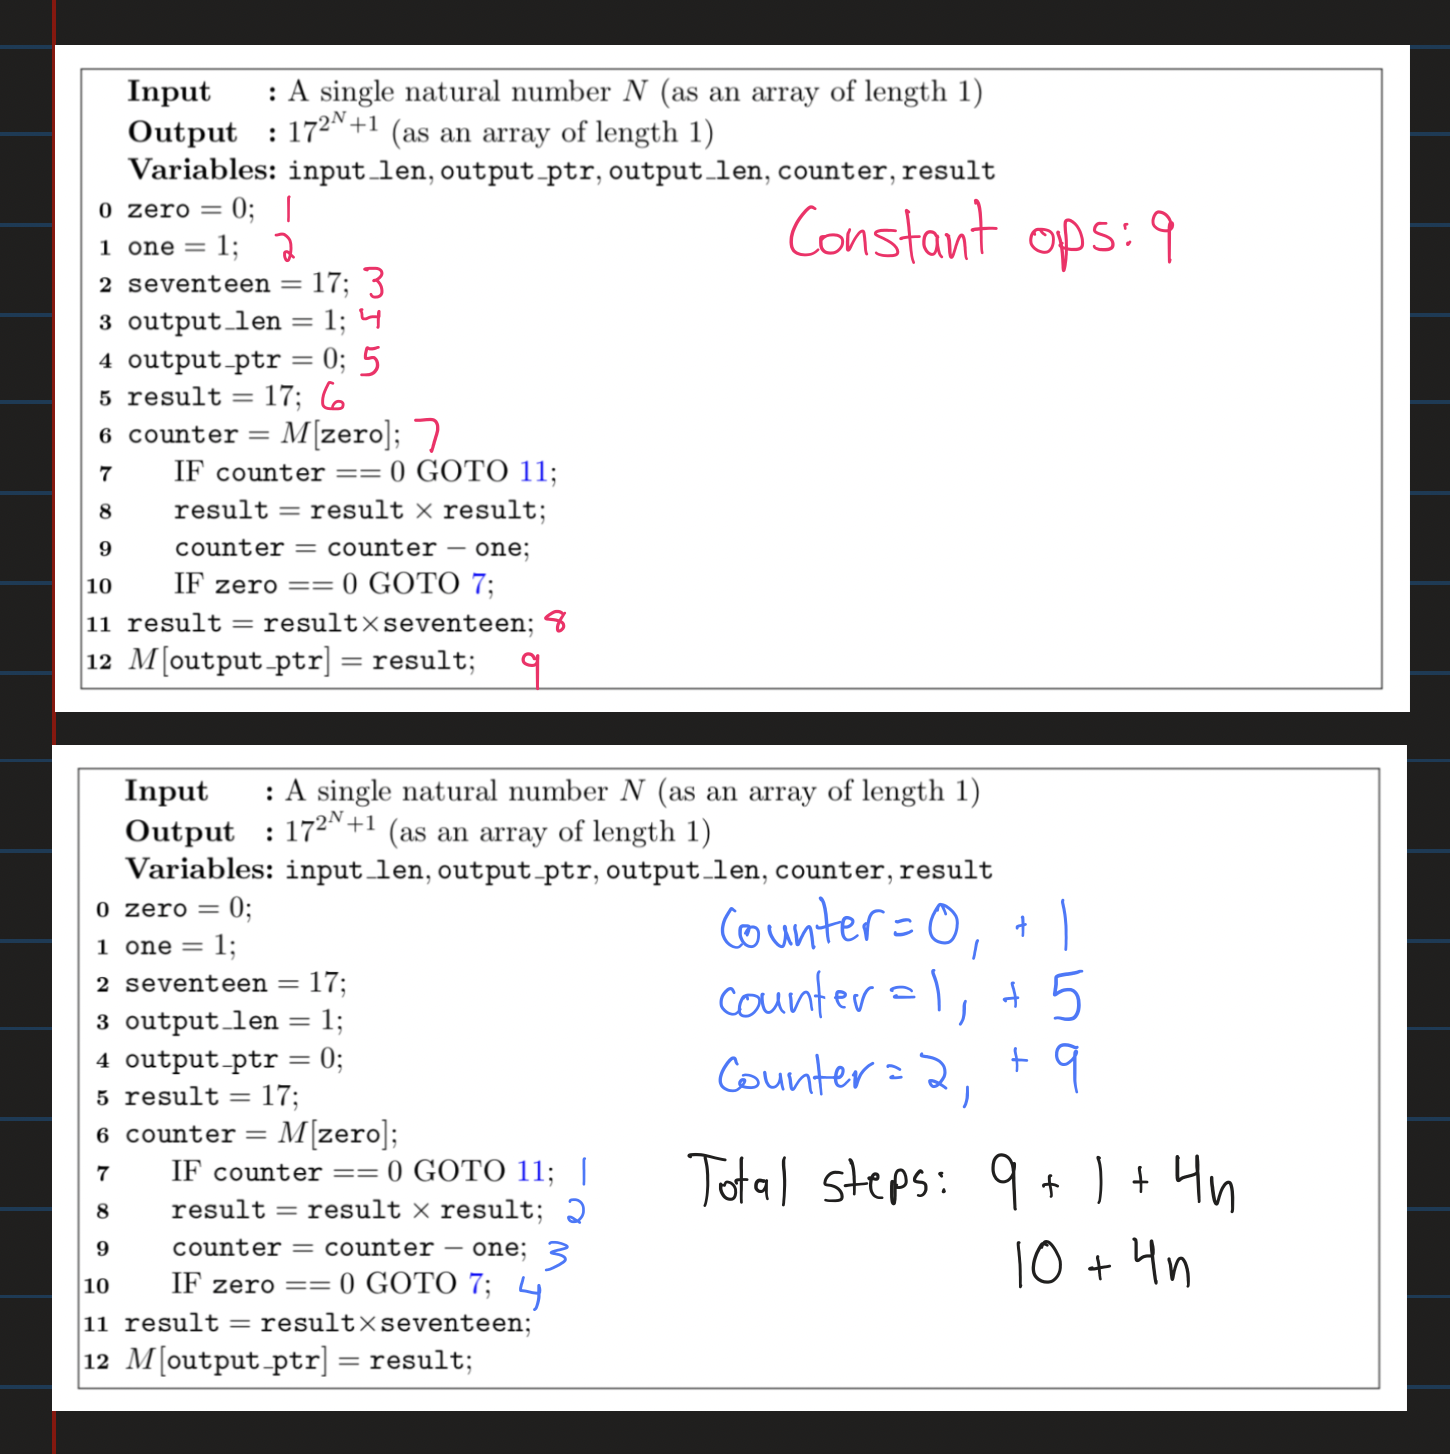
\includegraphics[scale=0.3]{work/2a 0.png}         
        \newline
        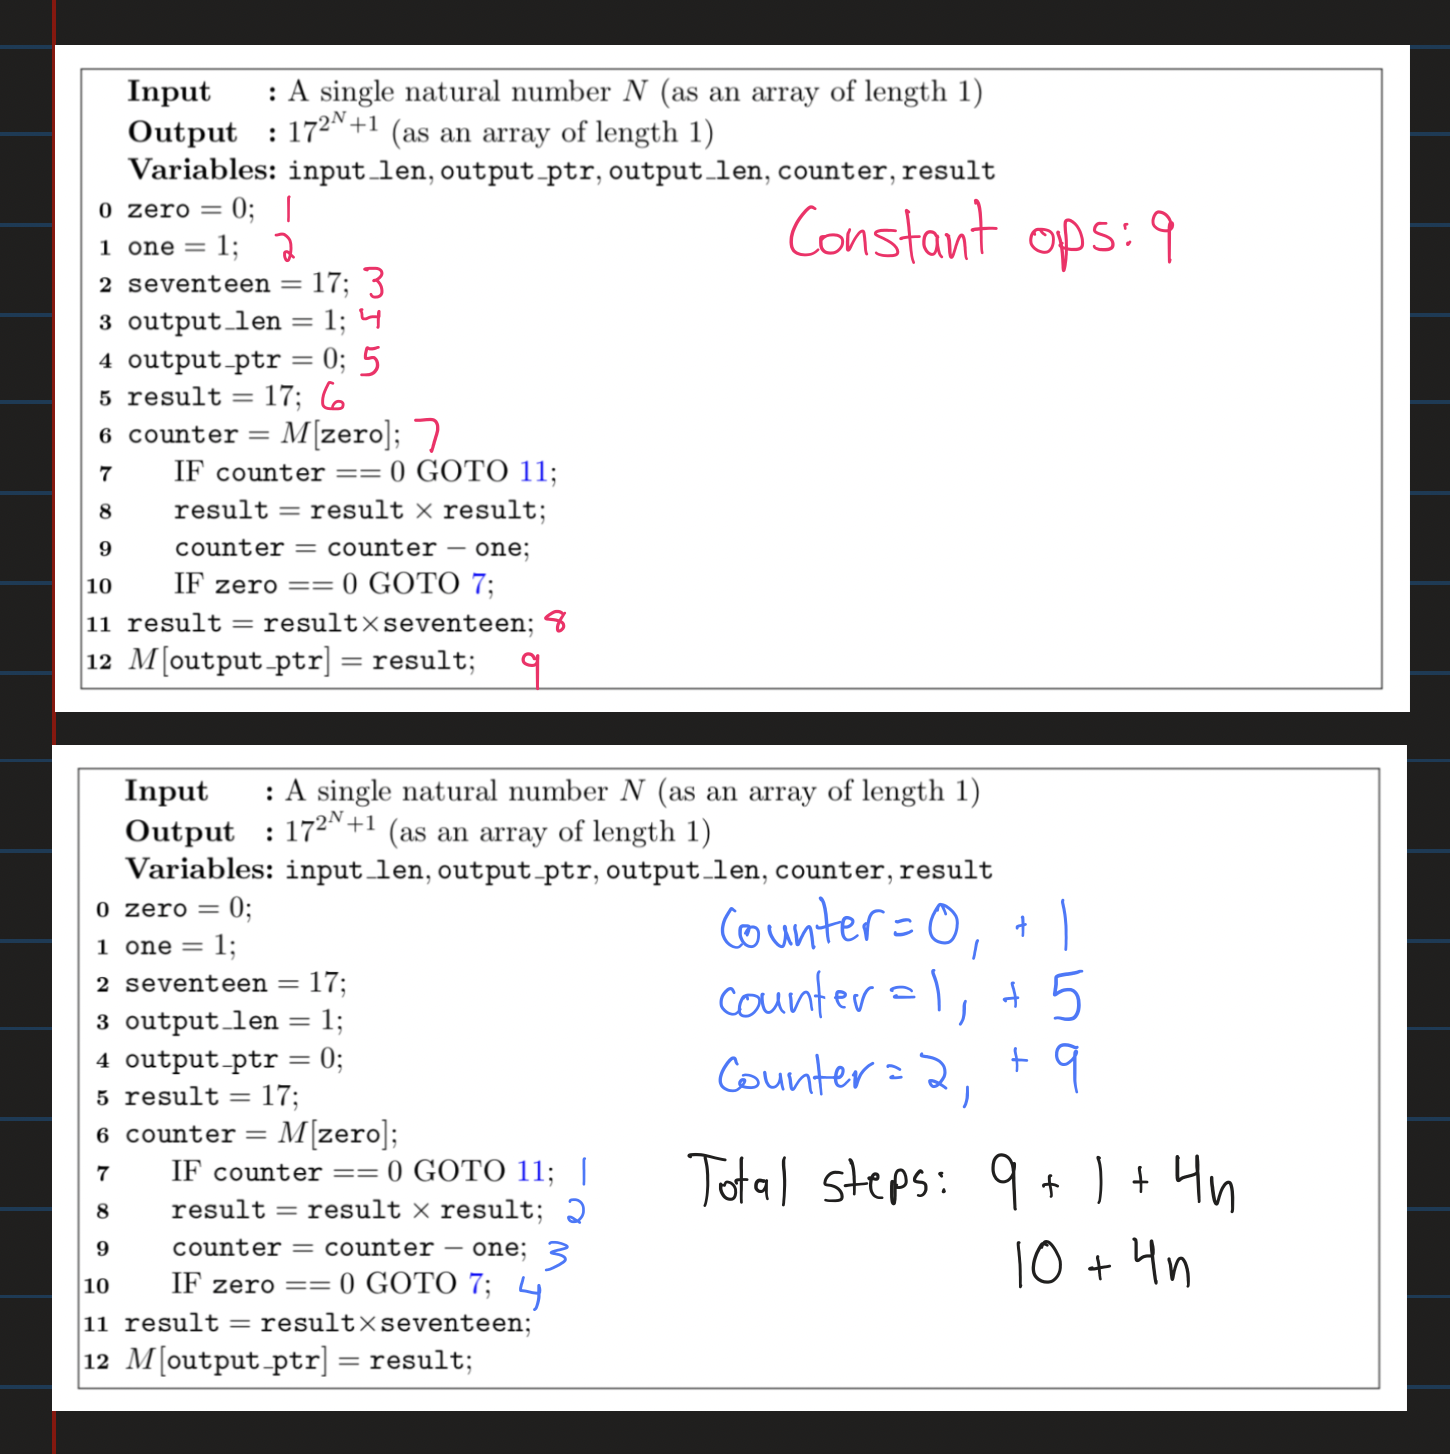
\includegraphics[scale=0.3]{work/2a 0.png}         
        \newline
        \newline
        RAM running time is a function of the number of basic operations performed. In terms of input length $n$, the first equation runs in about $f(n) = 10 + 4n$ steps, and the second equation runs in about $f(n) = 14 + 7n$ steps. Because the second equation has more baseline operations and has a higher linear growth factor, the second RAM program is slower and the first is faster.
    \end{quote}
    \item Using your RAM Simulator, run both RAM programs on inputs $N=0,1,2,\ldots,15$ and graph the actual running times (in clock time, not RAM steps).  (We have provided you with some timing and graphing code in the Github repository.) Which one is faster?  \label{itm:realtime}  
    \begin{quote}
        \color{purple}
        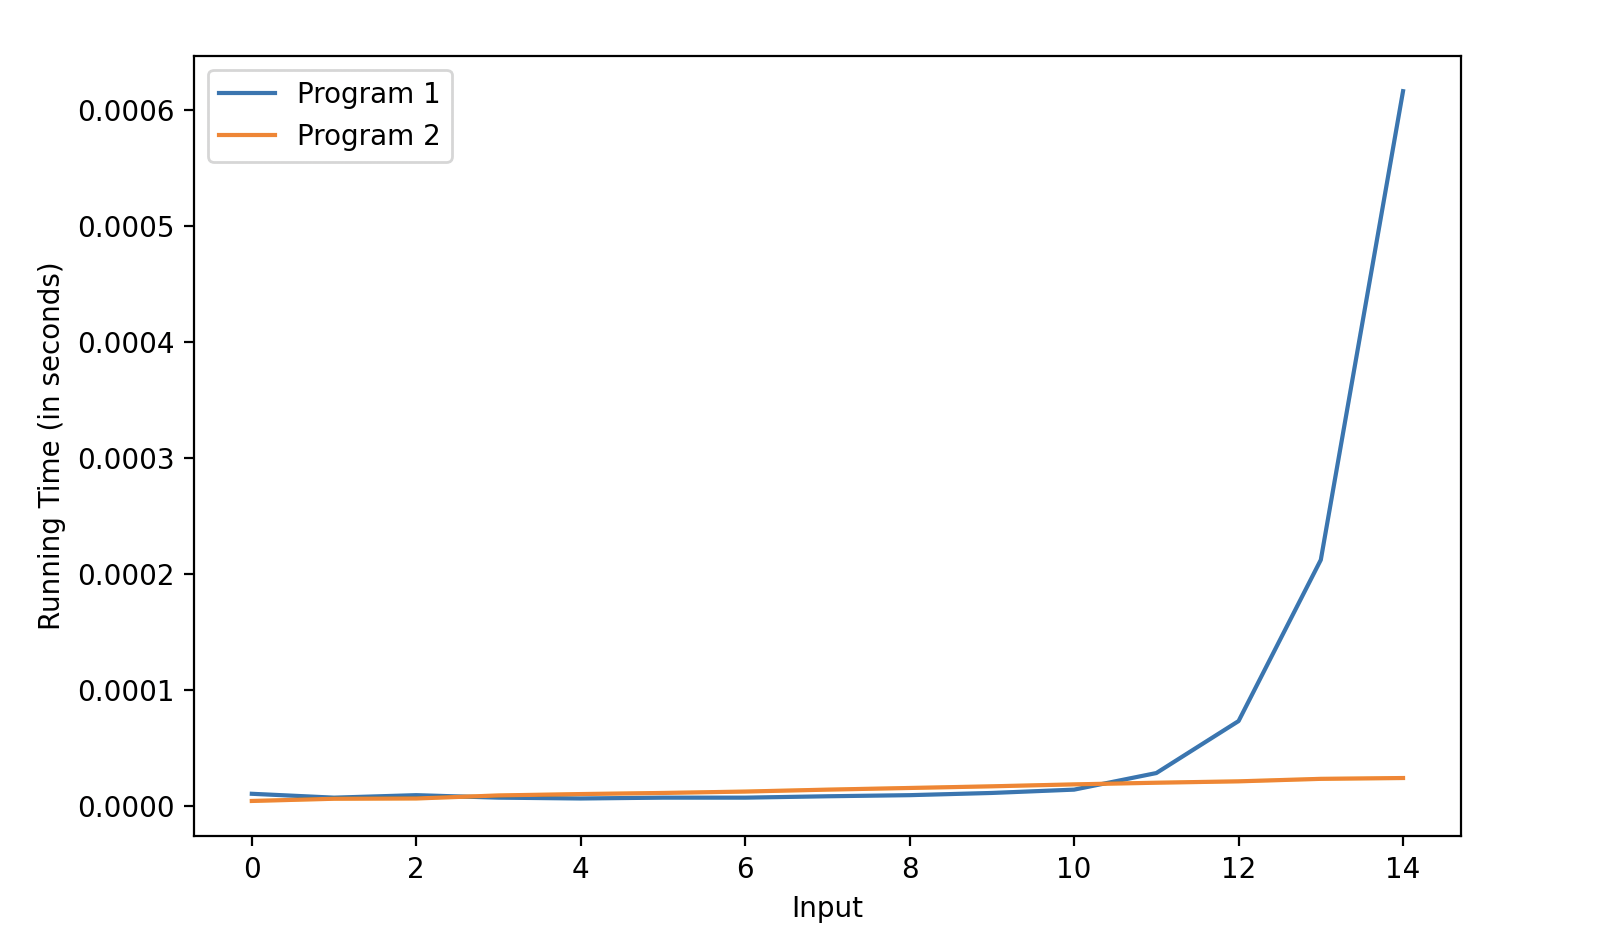
\includegraphics[scale=0.4]{work/2b.png}         
        \newline
        For inputs 0 through 10, performance is pretty much equal. However, for about $n \geq 10$, program 2 becomes much faster than program 1. (program 1 appears to grow at an asymptotically greater rate)
    \newline 
    \newline 
    \textbf{Program 1}: \newline 
    \begin{minted}{python}
prog1 = [
    8,
    ["assign", zero_id, 0],
    ["assign", one_id, 1],
    ["assign", seventeen_id, 17],
    ["assign", output_len_id, 1],
    ["assign", output_ptr_id, 0],
    # line 5
    ["assign", result_id, 17],
    # line 6
    ["read", counter_id, zero_id],
    # line 7
    ["goto", counter_id, 11],
    # line 8
    ["*", result_id, result_id, result_id],
    # TODO: lines 5-8 from pseudocode
    ["-", counter_id, counter_id, one_id],
    ["goto", zero_id, 7],
    ["*", result_id, result_id, seventeen_id],
    ["write", output_ptr_id, result_id],
] 
    \end{minted} 
    \vspace{1em}
    \textbf{Program 2}: \newline 
    \begin{minted}{python}
prog2 = [
    10,
    ["assign", zero_id, 0],
    ["assign", one_id, 1],
    ["assign", seventeen_id, 17],
    ["assign", output_len_id, 1],
    ["assign", output_ptr_id, 0],
    ["assign", result_id, 17],
    ["assign", W_id, 2**32],
    ["read", counter_id, zero_id],
    ["goto", counter_id, 15],
    ["*", result_id, result_id, result_id],
    ["/", temp_id, result_id, W_id],
    ["*", temp_id, temp_id, W_id],
    ["-", result_id, result_id, temp_id],
    ["-", counter_id, counter_id, one_id],
    # line 14
    ["goto", zero_id, 8],
    # line 15
    ["*", result_id, result_id, seventeen_id],
    # line 16
    ["/", temp_id, result_id, W_id],
    # line 17
    ["*", temp_id, temp_id, W_id],
    # line 18
    ["-", result_id, result_id, temp_id],
    # line 19
    ["write", output_ptr_id, result_id],
]
    \end{minted}
    \vspace{1em}
    \end{quote} 
    
    \item Explain the discrepancies you see between Parts~\ref{itm:RAMtime} and \ref{itm:realtime}.  (Hint: What do we know about the relationship between the RAM and Word-RAM models, and why is it relevant to how efficiently the Python simulation runs?) 
    \begin{quote}
        \color{purple}
        The program growth rates are different because of the size of the values the programs operate upon. \newline 
        Program 1 simulates a RAM model on hardware with implicit Word RAM constraints. Past about $n = 10$, the numbers being operated upon in Program 1 are massive and grow in length very quickly. In the RAM model, we can operate on arbitrarily-sized integers in constant time. However, Python operations on arbitrary-size integers are not constant because such large values cannot fit within a single register and are thus represented by arrays of smaller integers. Because of this, arithmetic operations slow down as the size of the numbers grows. Even the final step, returning a value, is affected. As noted by theorem 5.5 in the lecture notes, Program 1 has to return an arbitrarily-large output, which comes with its own runtime complexity. \newline
        In Program 2, the modulo operator prevents the values within the computation from ever exceeding $2^{32}$. This limits the length of any intermediate or output values to a length of about 10, which yields constant-time performance. Introducing this modulo operator is akin to setting the word size of our program to $32$ such that no arithmetic operation ever produces a result exceeding $2^{32}$. \newline 
        Thus, because of the size differences of the numbers being calculated in Program 1 and Program 2, Program 1 ultimately grows at a higher algorithmic rate than Program 2, which is exhibited by the graph.
    \end{quote}
    
    
    \item (optional\footnote{This problem won't make a difference between N, L, R-, and R grades.}) Give a theoretical explanation (using asymptotic estimates) of the shapes of the runtime curves you see in Part~\ref{itm:realtime}. You may need to do some research online and/or make guesses about how Python operations are implemented to come up with your estimates. 
    \begin{quote}
        \color{purple}
        It looks like Program 1 operates with linear time complexity, and it looks like Program 2 runs with some form of polynomial time complexity. \newline 
        If $n$ represents the input number, let $b$ represent the number of digits in the largest number ever computed within either program. In Program 2, $b$ is limited to a constant size by the modulo operator. So, arithmetic operations on numbers of length $b$ take constant time. Because of this, Program 2 achieves runtime complexity of $O(n)$. \newline 
        In Program 1, $b$ can grow to be arbitrarily large (it does). Python bignum multiplication uses Karatsuba's algorithm, which has runtime complexity of about $O(b^{1.58})$ (according to Wikipedia). Because this multiplication occurs for every iteration of the loop, Program 1 has runtime complexity of $O(n \cdot b^{1.58})$. The value of $b$ grows exponentially and dominates that of $n$, which explains why the runtime curve of Program 1 grows so much faster that of Program 2 after a certain point.
    \end{quote}
\end{enumerate}

\item (Simulating Word-RAM by RAM)  Show that for every Word-RAM program $P$, there is a RAM program $P'$ such that $P'$ halts on $x$ iff $P$ halts on $x$, and if they halt, then  $P'(x)=P(x)$ and 
       $$\Time_{P'}(x) = O\left(\Time_P(x)+n+w_0\right),$$
where $n$ is the length of $x$ and $w_0$ is the initial word size of $P$ on input $x$.  (This was stated without proof in Lecture Notes 7.) 

Your proof should use an {\em implementation-level} description, similar to our proof that RAM programs can be simulated by ones with at most $c$ registers.  Recall that Word-RAM programs have read-only variables $\memsize$ and $\wordlen$; you may want to start your simulation by calculating these variables as well as another variable representing $2^{\wordlen}$.  Then think about how each operation of a Word-RAM program $P$ can be simulated in a RAM program $P'$, taking care of any differences between their semantics in the Word-RAM model vs. the RAM model. Don't forget MALLOC!

\begin{quote}
    \color{purple}
     I'll prove the existence, correctness, and runtime of the RAM program by translating distinct Word RAM operations into their RAM counterparts. \newline 
     \newline
    First, let the RAM program initialize some constant number of pointers to memory for use in temporary calculations. Throughout the proof, I will abstract certain operations through these "temp" variables. Initializing, writing, or reading a temp variable requires constant time, so this doesn't affect overall runtime. \newline
    \newline
    \textbf{Assign \memsize, compute $maxVal$}: \newline
    The RAM program enters with access to a variable containing the length of the inputs. Let the RAM program initialize a constant address called $\memsize$ and write the length of inputs to it. Then, let the RAM program initialize another constant address called $maxVal$ as 0. Initialize a temp iteration variable to the first address of inputs and enter a GOTO loop that increments the temp variable and reads the value of each input address. Run the GOTO loop until the max input address minus the iteration variable is equal to zero (all inputs have been scanned). For each iteration, if the scanned input value exceeds $maxVal$, reassign $maxVal$ to be that input value. Once this GOTO loop exits, $maxVal$ will represent the greatest integer in the input sequence. This adds $O(inputLen)$ time complexity to the algorithm.
    \newline
    \newline
    \textbf{Compute and assign $\wordlen$ and $limit$}: \newline
    Next, let the RAM program initialize two more constant addresses called $\wordlen$ and $limit$. Assign $\wordlen = 0$ and $limit = 1$. Assign a temp variable to be $\memsize$ (in this paragraph, we'll call this temp variable $maxInput$). Then, read $maxVal$ and use a GOTO sequence to assign $maxInput$ to be $maxVal$ if $\memsize - maxVal$ is equal to zero. This ensures that $maxInput$ holds the greater of $\memsize$ and $maxVal$. Now, using GOTO statements and temp variables, construct a loop that runs until $maxInput - limit + 1 = 0$ (remembering that negative numbers are raised to zero). For each iteration of the loop, increment $\wordlen$ by one and reassign $limit$ to be itself times two. By the time the loop exits, $\memsize$ and $\wordlen$ should equal their counterparts in Word RAM, and $limit$ should be $2^\wordlen$. Assignment, GOTO, multiply, and increment are all constant time operations, and the operations execute $\wordlen$ times. This adds $O(\wordlen)$ time complexity to the algorithm.
    \newline
    \newline 
    Then, commands can be copied directly from the Word RAM to the RAM program, making the substitutions below as the appropriate tokens are identified: 
    \newline
    \newline
    \textbf{Memory tokens: read or write}: \newline 
    When a memory read or write is encountered, first retrieve the value of $\memsize$ from memory. If the requested address or value exceeds $\memsize$, proceed as if the operation had no effect. Otherwise, perform the memory read or write. This sequence requires an additional memory read into a temp variable and a GOTO command to execute the two cases, but this still permits constant time write and read operations. \newline 
    \newline
    \textbf{Arithmetic tokens: +, -, *, ÷}: \newline
    Before any operation, read the value of $limit$ into a temp variable. Then, perform the operation. If the result of the operation meets or exceeds $limit$, re-assign the operation result to be $limit - 1$. Because memory read and write as well as RAM arithmetic operations have constant time complexity, arithmetic in $P'$ still requires constant time.
    \newline \newline
    \textbf{Malloc}: \newline
    When $malloc$ is encountered, first read $\memsize$, $\wordlen$, and $limit$ into temp variables. Then, increment $\memsize$, and write the updated $\memsize$ back into memory. After that, set the memory location at $\memsize - 1$ equal to zero. If the updated value of $\memsize$ is now equal to $limit$, set the memory value of $limit$ to be itself times two and update $\wordlen$ to be itself plus one. Because each of these operations is constant time, $malloc$ also remains constant time.
    \newline
    \newline
    \textbf{Conclusions}: \newline
    For the sake of brevity, the reasoning above assumes certain operations and control flows like variable reassignment and GOTO looping to be implementation details. Allowing such assumptions, the operations explained above properly augment the RAM model to run any Word RAM program as if it were in a Word RAM environment. In doing so, the correctness of any Word RAM program $P$ is retained for the emulated RAM program $P'$.
    \newline
    \newline
    \textbf{Time complexity}: \newline
    The RAM program simulates a Word RAM program, so the RAM-simulated program has at least the runtime of the Word-RAM program, which is $O(T_p(x))$. The algorithm-specific runtime complexity is not affected because every Word RAM operation has the same complexity as its counterpart in the RAM simulation. \newline 
    The proper calculation of $\memsize$ and $\wordlen$ required additional time during the setup phase. Because $\wordlen$ must accommodate both the length of inputs and the maximum input value, we needed to iterate through every input value to find the maximum. This took $O(n)$ time. Then, the actual computation of $\wordlen$ required runtime $O(w_0)$. \newline 
    Together, these factors result in a worst case time complexity of $O(T_p(x) + n + w_0)$.
    
\end{quote}



\end{enumerate}


\end{document}
